% !TEX TS-program = XeLaTeX
% all document files must be coded in UTF-8
\documentclass{textolivre}

\journalname{Texto Livre: Linguagem e Tecnologia}
\thevolume{14}
\thenumber{1}
\theyear{2020}
\receiveddate{\DTMdisplaydate{2020}{08}{09}{-1}} % YYYY MM DD
\accepteddate{\DTMdisplaydate{2020}{10}{05}{-1}}
\publisheddate{\today}

\title{Competencia léxica y escritura académica: analíticas deaprendizaje en un curso de escritura universitaria}
\othertitle{Competência léxica e escrita acadêmica: análise da aprendizagem em um curso de escrita universitário}
\othertitle{Lexical competence and academic writing: learning analytics in a university writing course}

\author[1]{Gabriel Valdés-León}

\affil[1]{Universidad de Las Palmas de Gran Canaria, Espanha. Email: \url{gvaldesl@ucsh.cl}. \orcid{0000-0001-8807-8838}}

% Corresponding author
\corrauthor{Gabriel Valdés-León}

% DOI
\articledoi{10.35699/1983-3652.2021.24560}

% Abbreviated author list for the running footer
\runningauthor{Valdés-León, G.}

%\usepackage[backend=biber,style=abnt, ittitles]{biblatex}
%\DeclareLanguageMapping{brazil}{brazil-apa}
\addbibresource{article.bib}     
% use biber instead of bibtex
% $ biber tl-article-template
% $ pdflatex tl-article-template.tex

% set language of the article
\setdefaultlanguage{spanish}
\setotherlanguage{portuguese}
\setotherlanguage{english}

\begin{document}
\maketitle

\begin{poliabstract}
\begin{abstract}
Gracias a la generación de analíticas de aprendizaje, se recogió
informaciónrelacionada con el desempeño léxico y escritural en 36 textos
producidos por estudiantespertenecientes a un curso de escritura de educación
superior. Esta información no solopermitió tomar decisiones pedagógicas en el
corto plazo, sino también planificar unainvestigación que indagara en la
relación que existe entre ambas competencias. Elartículo que aquí se presenta
se hace cargo del segundo desafío planteado, y tiene comoobjetivo identificar
la relación que existe entre el dominio léxico académico y el nivel de
lostextos producidos por este grupo de alumnos a partir de las analíticas de
aprendizajeobtenidas. Para ello, se elaboró un estudio de caso, de tipo
preexperimental y transversal,en el que se compara la calidad de los textos
redactados por los discentes en una tareade escritura con un estudio
lexicométrico realizado a esos mismo escritos utilizando elsoftware libre
Iramuteq. Los resultados indican que existe una estrecha relación entreléxico
académico y calidad del contenido, pero que el vínculo se vuelve
menosdeterminante al contrastar léxico académico con la calidad textual de los
trabajos.

\keywords{Competencia léxica \sep Escritura académica \sep Analíticas de aprendizaje \sep Iramuteq \sep Análisis lexicométrico.}
\end{abstract}

\begin{portuguese}
\begin{abstract}
Graças à geração de análises de aprendizagem, informações relacionadas
aodesempenho lexical e escritural foram coletadas em 36 textos produzidos por
alunos deum curso de redação de ensino superior. Essas informações
possibilitaram não apenastomar decisões pedagógicas em curto prazo, mas também
planejar um estudo queinvestigasse a relação entre as duas competências. O
artigo aqui apresentado trata dosegundo desafio que se coloca, e tem como
objetivo identificar a relação que existe entreo domínio lexical acadêmico e o
nível dos textos produzidos por este grupo de alunos apartir das análises de
aprendizagem obtidas. Para tanto, foi desenvolvido um estudo decaso, do tipo
pré-experimental e transversal, no qual a qualidade dos textos escritos
pelosalunos em uma tarefa de escrita foi comparada com um estudo lexicométrico
realizadosobre essas mesmas escritas no software livre Iramuteq. Os resultados
indicam queexiste uma estreita relação entre o léxico acadêmico e a qualidade
do conteúdo, mas quea vinculação se torna menos decisiva ao contrastar o léxico
acadêmico com a qualidadetextual dos trabalhos.

\keywords{Competência lexical \sep Escrita acadêmica \sep Análises de aprendizagem \sep Iramuteq \sep Análise lexicométrica.}
\end{abstract}
\end{portuguese}

\begin{english}
\begin{abstract}
Based on learning analytics, information related to lexical and
scripturalperformance was collected in 36 texts produced by students belonging
to a highereducation writing course. This information not only allowed to make
pedagogical decisionsin the short term, but also to plan an investigation on
the relationship between bothcompetences. The article presented here addresses
the second challenge posed, and itsobjective is to identify the relationship
that exists between the academic lexical domainand the level of the texts
produced by this group of students based on the learninganalytics obtained. To
do this, a case study was developed, of a pre-experimental andcross-sectional
type, in which the quality of the texts written by the students in a
writingtask is compared with a lexicometric study carried out on those same
writings using thefree software Iramuteq. The results indicate that there is a
close relationship betweenacademic lexicon and content, but that link becomes
less decisive when contrastingacademic lexicon with textual quality.

\keywords{Lexical competence \sep Academic writing \sep Learning analytics \sep Iramuteq \sep .Lexicometric analysis.}
\end{abstract}
\end{english}

\end{poliabstract}


\section{Introducción}\label{sec-intro}

La utilización de analíticas de aprendizaje para mejorar los procesos
educativosposee ya un par de décadas, no obstante, la investigación en torno a
su uso se encuentraen pleno auge \cite{caceres2020}. Pese a lo alentador que
esto último puedaparecer, existe aún una considerable distancia entre los
avances de la tecnología y elámbito educativo, lo que representa un profundo
desaprovechamiento del potencial quetienen las tecnologías de uso diario en el
aprendizaje de los estudiantes, en elmejoramiento de los métodos didácticos y
en la respuesta que espera la sociedad de lasinstituciones educativas \cite[p. 556]{penalvo2015}. 
Esta distancia se haceaún más patente en espacios formativos
como los que ofrece Sudamérica, por ejemplo,en donde la incorporación de la
tecnología a la educación es aún una tarea pendiente.

Efectivamente, la implementación generalizada de entornos
completamentetecnologizados en las aulas del sur de América, al estilo de los
Entornos Virtuales deAprendizaje (EVA), parece un sueño aún bastante alejado;
no obstante, sin dejar de ladoiniciativas de alta envergadura, como el proyecto
LALA, orientado hacia el uso deanalíticas de aprendizaje para mejorar la
educación superior de América Latina, es posibleencontrar en la literatura
especializada experiencias que dan cuenta de resultadosexitosos que,
generalmente, se encuentran circunscritos a la enseñanza de un tema o decurso
en particular \cite[por ejemplo]{ninoCarrasco2019}.

Actualmente, las analíticas de aprendizaje suelen definirse como un proceso
demedición del comportamiento de los estudiantes en entornos virtuales con el
fin derealizar un seguimiento de su desempeño y, gracias a ello, crear data que
permita tomardecisiones pedagógicas. En palabras de \textcite{Sabulsky2019},
“las analíticas deaprendizaje son dispositivos tecnológicos que se incorporan a
entornos virtuales deinteracción, con el fin de registrar las huellas digitales
que dejan quienes participan enellos, creando grandes bases de datos”.

Si bien la definición anterior sitúa a las analíticas de aprendizaje
inevitablemente
dentro de entornos virtuales, esta investigación adopta una
perspectiva un tanto másamplia, pues las concibe como herramientas que
“procesan datos, analizan estadísticas,generan informes de uso y
proporcionan a profesores y alumnos información sobre
lasinteracciones del alumno y de su progresión” \cite[p. 185]{conole}. Esto
nos permiteconsiderar que los datos recogidos luego de la experiencia de aula
que forma parte deeste estudio, la que se realizó de manera presencial y con
metodologías de aprendizaje'tradicionales' (es decir, sin estar inmersos en un
EVA), pueden enriquecerse con análisisestadísticos proporcionados por
herramientas tecnológicas. Gracias a ello, la informaciónque se ha
obtenido luego del desarrollo de una tarea de escritura por
parte de los 36estudiantes del curso Producción oral y escrita ha sido
analizada desde dos perspectivas:desempeño escritural y desempeño léxico.

Este trabajo se enmarca en los continuos esfuerzos de una universidad
chilenaprivada por aportar en la formación de los estudiantes de Pedagogía en
castellano através de la búsqueda permanente de mecanismos de innovación
docente. Como partede esos esfuerzos, este trabajo tiene como objetivo
identificar la relación que existe entreel dominio léxico académico y el nivel
de los textos producidos por estudiantes de nuevoingreso a partir de las
analíticas de aprendizaje obtenidas. Para ello, se diseñó un estudiode caso que
contó con la participación de la totalidad de los estudiantes de primer año
dedicha carrera (36 matriculados, año 2019), en el que se analizó información a
través dedos mecanismos: una rúbrica para conocer tanto el nivel de redacción
como el dominio decontenidos; y un análisis lexicométrico llevado a cabo a
través del programa informáticoIramuteq, que permitió conocer el manejo del
léxico académico por parte de losestudiantes.


\subsection{La escritura y su relación con el léxico}\label{sec-la-escr}
La escritura es un proceso complejo que va mucho más allá de garabatear
signossobre un papel. Es una competencia transversal, por tanto, transferible,
que implica unesfuerzo multidimensional (pues contempla los niveles cognitivo,
social e inclusoemocional) y que se desarrolla durante toda la vida \cite{Balta2018}.
En este sentido, laescritura – como proceso – involucra una serie de
habilidades que adquieren mayor omenor relevancia dependiendo de la situación
comunicativa en la que se encuentra elhablante y del texto – o producto – que
se quiere elaborar. Así, un texto académicorequiere investigar, ordenar,
clasificar, jerarquizar, criticar, adecuar, evaluar..., mientrasque textos que
dejan en un segundo plano el valor epistémico de la escritura resultan sermenos
demandantes, al menos en el plano cognitivo \cite{cantis2013,navarro}

La importancia medular que tienen tanto la lectura como la escritura para
eldesarrollo humano y, particularmente, para la educación, ha motivado una
considerablecantidad de investigaciones sobre estrategias que permitan
fortalecer estascompetencias. Si nos enfocamos en los estudios realizados en
educación superior en elámbito latinoamericano, es posible identificar “un
aumento progresivo de iniciativas deenseñanza, investigación, publicación,
eventos y esfuerzos de sistematización”\cite{Navarro2016}.

Esta creciente preocupación por los estudios de alfabetización académica
sefundamenta, entre otros aspectos, en el desafío que una nueva cultura
discursiva supone
\begin{quote}
El concepto de alfabetización académica [...] señala el conjunto de nociones
yestrategias necesarias para participar en la cultura discursiva de las
disciplinas asícomo en las actividades de producción y análisis de textos
requeridas paraaprender en la universidad. Apunta, de esta manera, a las
prácticas de lenguaje ypensamiento propias del ámbito académico \cite[p. 410]{cantis2003}.
\end{quote}

Este nuevo escenario plantea también nuevos desafíos en el plano discursivo,
loque puede desembocar en problemas de rendimiento académico. En
efecto,investigaciones como las de \textcite{Ayala2019,ValdsLen2020} 
señalan que losestudiantes universitarios de primer año suelen evidenciar
debilidades respecto de suscompetencias de lectura y escritura al momento de
hacer frente estas nuevas demandasde la educación terciaria. Y uno de los
caminos que surgen desde la didáctica de laescritura puede encontrarse en el
fortalecimiento de las (sub)competencias comunicativasasociadas a la escritura,
entre ellas, la lectura y el léxico.

Los estudios que abordan el léxico como parte de la competencia
comunicativatambién han evidenciado un aumento sostenido de publicaciones
académicas queestudian tópicos relacionados con la didáctica, la evaluación y
el aprendizaje delvocabulario \cite{perfetti2001,rufat2016}. No
obstante, al momentode revisar lo que se ha producido en el área, queda en
evidencia que la mayor cantidadde estudios que buscan potenciar la competencia
léxica han surgido bajo el alero de laenseñanza del español como lengua
extranjera (ELE), siendo considerablemente menorel número de trabajos que
apuntan hacia la enseñanza del español como lengua materna.Por su parte,
subdisciplinas lingüísticas como la disponibilidad léxica y la
psicolingüísticaexperimental se han enfocado en temas más acotados como la
medición del léxicodisponible y del léxico pasivo, sin relacionar
necesariamente sus resultados con el ámbitoeducativo \cite{GermanyG2000,echeverria1987,RiffoOcares2014}.

Lo anterior no es más que una evidencia de que la posición protagónica que
hatomado la competencia léxica como parte de la competencia comunicativa ha
sidoreconocida por los docentes de ELE, pero no suficientemente valorada cuando
se trata dedidáctica del español como lengua materna, por lo que nos parece que
es un ámbito queresulta necesario fortalecer, sobre todo, considerando los
datos que existen cuandorelacionamos competencia léxica, competencias lectoras
y competencias escriturales \cite{GonzaloZapico2016,Zapico2017,kaur,Pinto2019}.

En el plano local chileno, basta con observar los resultados que se han
obtenidotanto en evaluaciones estandarizadas nacionales (e.g., SIMCE) como
internacionales (e.g., PISA) \cite{VillarroelHenrquez2015,FigueroaSeplveda2018}
paracomprender la necesidad de reforzar los procesos relacionados
con lectura y escritura anivel primario, secundario y terciario y,
específicamente, con la formación de los futurosdocentes, con énfasis en los
profesores de español como lengua materna.

Hasta este punto, hemos mencionado la importancia que tiene el léxico dentro de
laenseñanza de una lengua, ya sea lengua materna o una segunda lengua, por
ello, resultaimprescindible profundizar en torno a esta competencia.

Existe consenso entre los investigadores especializados en el estudio del
léxico en mencionar a Richards como uno de los primeros lingüistas que abordó
el concepto decompetencia léxica, aunque cabe precisar que el autor utilizó la
expresión knowing aWord al momento de desarrollar su trabajo \cite{Richards1976,Choudhury2015,Velsquez2016}.
No obstante, más allá de la nomenclatura
utilizada, la propuesta deRichards fue pionera al momento de estudiar cómo las
palabras se relacionan de maneracompleja a nivel gramatical, semántico,
sociolingüístico y psicolingüístico \cite{catalan2002}, considerando
también elementos cognitivos, por cierto, dada laperspectiva pedagógica que su
obra posee. De esta manera, \textcite[p. 78--83]{Richards1976} propone ocho premisas que
permitirían guiar procesos de enseñanza de vocabulario:

\begin{enumerate}
\item El vocabulario de un hablante nativo continúa expandiéndose durante su adultez.
\item Conocer una palabra significa conocer el grado de probabilidad de encontrarla yasea de manera oral o escrita.
\item Conocer   una   palabra   implica   conocer   las   limitaciones   impuestas   a   su   uso   deacuerdo con las variaciones de función y situación.
\item Conocer una palabra significa conocer el comportamiento sintáctico asociado conesa palabra.
\item Conocer una palabra implica conocer su forma subyacente y las derivaciones quede esta palabra pueden surgir.
\item Conocer una  palabra implica conocer la red de  asociaciones entre  esa  palabra  yotras palabras de la lengua.
\item Conocer una palabra significa conocer el valor semántico de esa palabra.
\item Conocer una palabra significa conocer muchos de los otros significados asociadoscon esa palabra. [la traducción es nuestra]
\end{enumerate}

Como podemos observar, la propuesta de este autor destaca por romper con
unamirada estática frente al estudio del léxico, pues es enfático en señalar
que el aprendizajedel vocabulario no se limita al conocimiento del significado,
forma y derivados de unapalabra.

Sin dejar de valorar el aporte de Richards, \textcite[p. 15]{arancibia} menciona
que “[Richards] no distingue entre los diferentes niveles y grados de
conocimiento de lapalabra, ni tampoco menciona cómo el aprendiente llega a
adquirir ese conocimiento”. Fue \textcite{natio1990} quien realiza una propuesta en la
que establece una distinción explícitaentre el conocimiento receptivo y
productivo del vocabulario, señalando que el nivelproductivo involucra niveles
de conocimiento más altos \cite{Choudhury2015}. En estalínea de pensamiento,
\textcite{natio2001} amplía su propuesta y señala que lo queactualmente comprendemos
como competencia léxica implica tres niveles deconocimiento:

\begin{quote}
The terms receptive and productive apply to a variety of kinds of
languageknowledge and use. When they are applied to vocabulary, these terms
cover all theaspects of what is involved in knowing a Word. [...]. At the most
general level,knowing a word involves form, meaning and use \cite[p. 40]{natio2001}.
\end{quote}

En las diferentes definiciones que podemos encontrar en la literatura
especializadarespecto del concepto de competencia léxica, es posible observar,
con mayor o menorpreponderancia, la presencia de estos elementos. Así, por
ejemplo, \textcite[p. 57]{molina2007} define competencia léxica como la
“habilidad para reconocer y usar las palabras de una lengua del mismo modo que
los hablantes nativos lo hacen. Incluye, portanto, la comprensión de las
diferentes relaciones entre las familias de palabras y lascolocaciones comunes
de las palabras”. En esta misma obra, la autora refiere al trabajode \textcite[p. 152]{catalan2002},
quien señala que la competencia léxica implica, por
unaparte, conocer una palabra para poder utilizarla y, por otra, reconocerla y
relacionarla conlas demás, tanto en la oralidad como en la escritura. Es
innegable, entonces, que lacompetencia léxica es multidimensional y compleja y
-- tal como señalaba Richardsdécadas atrás-involucra un proceso de aprendizaje
progresivo.



\section{Metodología}\label{sec-metodologia}
A continuación, se exponen los principales elementos que conforman
lametodología de este estudio de caso en el que participaron 36 estudiantes
universitarioschilenos.

\subsection{Diseño}\label{sec-diseno}
El diseño de esta investigación se corresponde con un estudio preexperimental
detipo transversal, ya que que el trabajo se orienta hacia la descripción y el
análisis devariables tal como se presentan en un momento dado, considerando
incluso susinterrelaciones \cite{acuna2006}.

\subsection{Participantes}\label{sec-participantes}
Los criterios de inclusión consideraron, por una parte, la pertenencia al
cursoProducción oral y escrita I, en el que estaban inscritos la totalidad de
los estudiantes deprimer año cohorte 2019; por otra, la disposición de los
estudiantes por sumarse a esteestudio, lo que se tradujo en la aceptación por
escrito mediante un consentimientoinformado. En consecuencia, la investigación
contó con la participación de 36 jóvenesuniversitarios de entre 17 y 26 años.
La actividad curricular en la que se enmarcó eltrabajo posee carácter
obligatorio y se caracteriza por tributar a las competenciastransversales y
disciplinares del perfil de egreso de la titulación.

\subsection{Actividades pedagógicas}\label{sec-actividades}
Al finalizar el primer semestre del año 2019, la universidad en la que se
realizó estainvestigación solicitó a las unidades académicas la implementación
de una evaluaciónfinal de carácter integrativo, que permitiera recoger
información relacionada con el nivelde logro alcanzado en el desarrollo de
competencias declaradas en los programas decada actividad curricular. A raíz de
esto, el desafío para la Escuela de Educación enCastellano fue diseñar
evaluaciones que recogieran información en dos dimensiones:disciplinar, tanto
para lingüística y literatura como para los cursos pedagógicos y deformación
general; transversal, para conocer el nivel de desempeño en competenciasclave,
a saber, lectura y escritura.

Los resultados que expone esta investigación han sido obtenidos desde un corpus
de textos producidos por los 36 estudiantes de la cohorte al momento de rendir
laevaluación integrativa del curso Producción oral y escrita I. Esta evaluación
se dividió endos partes: la primera, que contenía preguntas de alternativas con
selección única,relacionadas con aspectos conceptuales abordados durante el
semestre; la segunda, queinvitaba a los estudiantes a elaborar un texto de
opinión a partir de la lectura de unfragmento (páginas 15-22) de Recetas para
escribir, de Daniel Cassany y Antonio García. Esta última sección fue la que se
recopiló para construir el corpus, pues permitió recogerinformación sobre
producción textual y léxico académico.


\subsection{Variables}\label{sec-variables}
Al momento de examinar los trabajos, se analizó la presencia de léxico
académico,por una parte, y la calidad de los textos, por otra. Para este último
aspecto, se tomaron encuenta “dominios disciplinares” y “criterios de
producción textual”, aspectos que se detallarán en el \Cref{sec-instru}. Por tanto,
se indagará en la relación entre dominio léxico académico y a) calidad textual
(o, en palabras simples, forma); b) contenido académico (contenido); y c) y
calidad global del texto (forma y contenido).


\subsection{Instrumento}\label{sec-instru}
Los instrumentos utilizados para la recolección y análisis de los datos son
aquellosque se relacionan con la evaluación de la actividad pedagógica. En
primer lugar,mencionaremos el segundo ítem de la evaluación integrativa
referida con anterioridad (ver \Cref{sec-actividades}), en el que se solicita a los estudiantes la
redacción de un texto de opinión apartir de una lectura académico. En segundo
lugar, para la revisión de la calidad de lostextos, se aplica una rúbrica que
toma como base la propuesta del Instituto Vasco deEducación \cite{ivei2013}
y, a partir de ahí, se revisa y
adapta por cuatro académicos de la Escuela deEducación en Castellano, cada uno
de los cuales la utiliza en sus respectivas actividadescurriculares. Luego de
esto, el instrumento se divide en dos grandes secciones, a saber,criterios para
la producción textual y dominio disciplinar, y cada uno de ellos se
subdividecomo se expone en el Cuadro 1:

%%%%%%%%%%%%%%%%%%%%%
% quadro 1
%%%%%%%%%%%%%%%%%%%%%

Esta distinción permite analizar la relación entre los resultados globales, por
unaparte, y los resultados obtenidos en cada nivel (disciplinar y formal), por
otra, yrelacionarlos, a su vez, con el nivel de competencia léxica.



\section{Proceso de análisis de datos}\label{sec-proc-ana}
Para procesar la información a nivel textual, se aplicó la rúbrica a cada
documentopor parte de dos especialistas en producción escrita y,
posteriormente, se utilizó elpromedio como mecanismo para resolver eventuales
diferencias de criterio al momentode evaluar \cite[p. 99]{gamboa2010}. Luego,
los resultados se organizaron atendiendo ala relación entre variables antes
establecida: calidad del contenido, calidad de laproducción, calidad global.

Por su parte, el procesamiento de los datos relacionados con la competencia
léxicase realizó a través de la selección de palabras clave obtenida de un
fragmento deRecetas para escribir, de Daniel Cassany y Antonio García, el cual
sirvió de base a losestudiantes para elaborar su escrito. Esta selección fue
realizada por tres especialistas,dos de ellos en lingüística y uno en didáctica
de la lengua, quienes elaboraron una lista depalabras que sirvió como
referencia para evaluar la competencia léxica académica, puesla presencia o
ausencia de cada pieza léxica incidió en el puntaje asignado. Se otorgó
elpuntaje total al texto que poseyó mayor cantidad de léxico académico y, a
partir de esabase, se puntuaron el resto de los escritos. Al respecto, cabe
señalar que los datosrelacionados con el léxico se obtuvieron específicamente
para esta investigación, por loque no incidieron en la calificación de los
estudiantes.

Una vez establecida esta lista de palabras, la información se procesó con
elprograma informático Iramuteq y los resultados se graficaron con ayuda de
Calc,programa de ofimática de acceso abierto. Respecto del primer software
mencionado, cabeseñalar que este también posee carácter libre y gratuito, y
“permite diferentes formas deanálisis estadísticos sobre corpus textuales y
sobre tablas de palabras por individuos [traducción propia]” \cite[p. 513]{Camargo2013}.
Tal como señalamos en \Cref{sec-intro}, losresultados que este programa
entrega, en tanto orientados hacia la educación, puedenser considerados como
‘analíticas de aprendizaje’, pues Iramuteq ofrece información quepermite tomar
decisiones pedagógicas fundamentadas que resultan útiles tanto paradocentes
como para estudiantes. En este sentido, hay que considerar que este programano
ha sido diseñado con esa intención, no obstante, los datos que proporciona
resultanvaliosos para enriquecer procesos pedagógicos.



\section{Resultados}\label{sec-resultados}
Con la finalidad de presentar este acápite de forma clara y ordenada,
hemosestandarizado todos los resultados, tanto los de producción como los de
léxico, en unaescala de porcentajes. Esto no solo favorece la presentación de
los datos, sino tambiénpermite comparar cada dimensión.

Organizaremos este apartado en cuatro secciones: en primer lugar,
presentaremosuna nube de palabras que da cuenta de la frecuencia de aparición
del léxico académicoen los textos revisados; después, abordaremos la relación
entre léxico académico y losresultados globales en escritura; luego, entre
léxico académico y contenido de los textos;y, por último, entre léxico
académico y calidad textual.


\subsection{Léxico académico}\label{sec-lex}
Cabe precisar que “la noción de léxico académico presupone la idea de
quealgunas unidades léxicas son usadas más frecuentemente en textos académicos
ydisciplinares que en textos pertenecientes a otras actividades sociales”
\cite[p. 251]{CisnerosEstupian2019}. En cuanto al método utilizado para medir el
léxico presente en losescritos de los estudiantes, se recurrió al criterio
experto de tres especialistas para laelaboración de una lista de palabras que
sirvió como baremo para evaluar el dominio léxico académico (ver \Cref{sec-proc-ana}). A partir
de esta lista, se elaboró una nube de palabras (\Cref{fig01}) que da cuenta de la
frecuencia de aparición en el total del corpus seleccionado. Estetipo de
representaciones resultan muy útiles en procesos de enseñanza-aprendizaje,
puespermiten evidenciar que, en casos como el que aborda esta investigación,
hay conceptosclave que efectivamente aparecen con muchísima frecuencia, lo que
favorece una visiónsobre qué aspectos resulta necesario potenciar.

\begin{figure}[htbp]
 \centering
 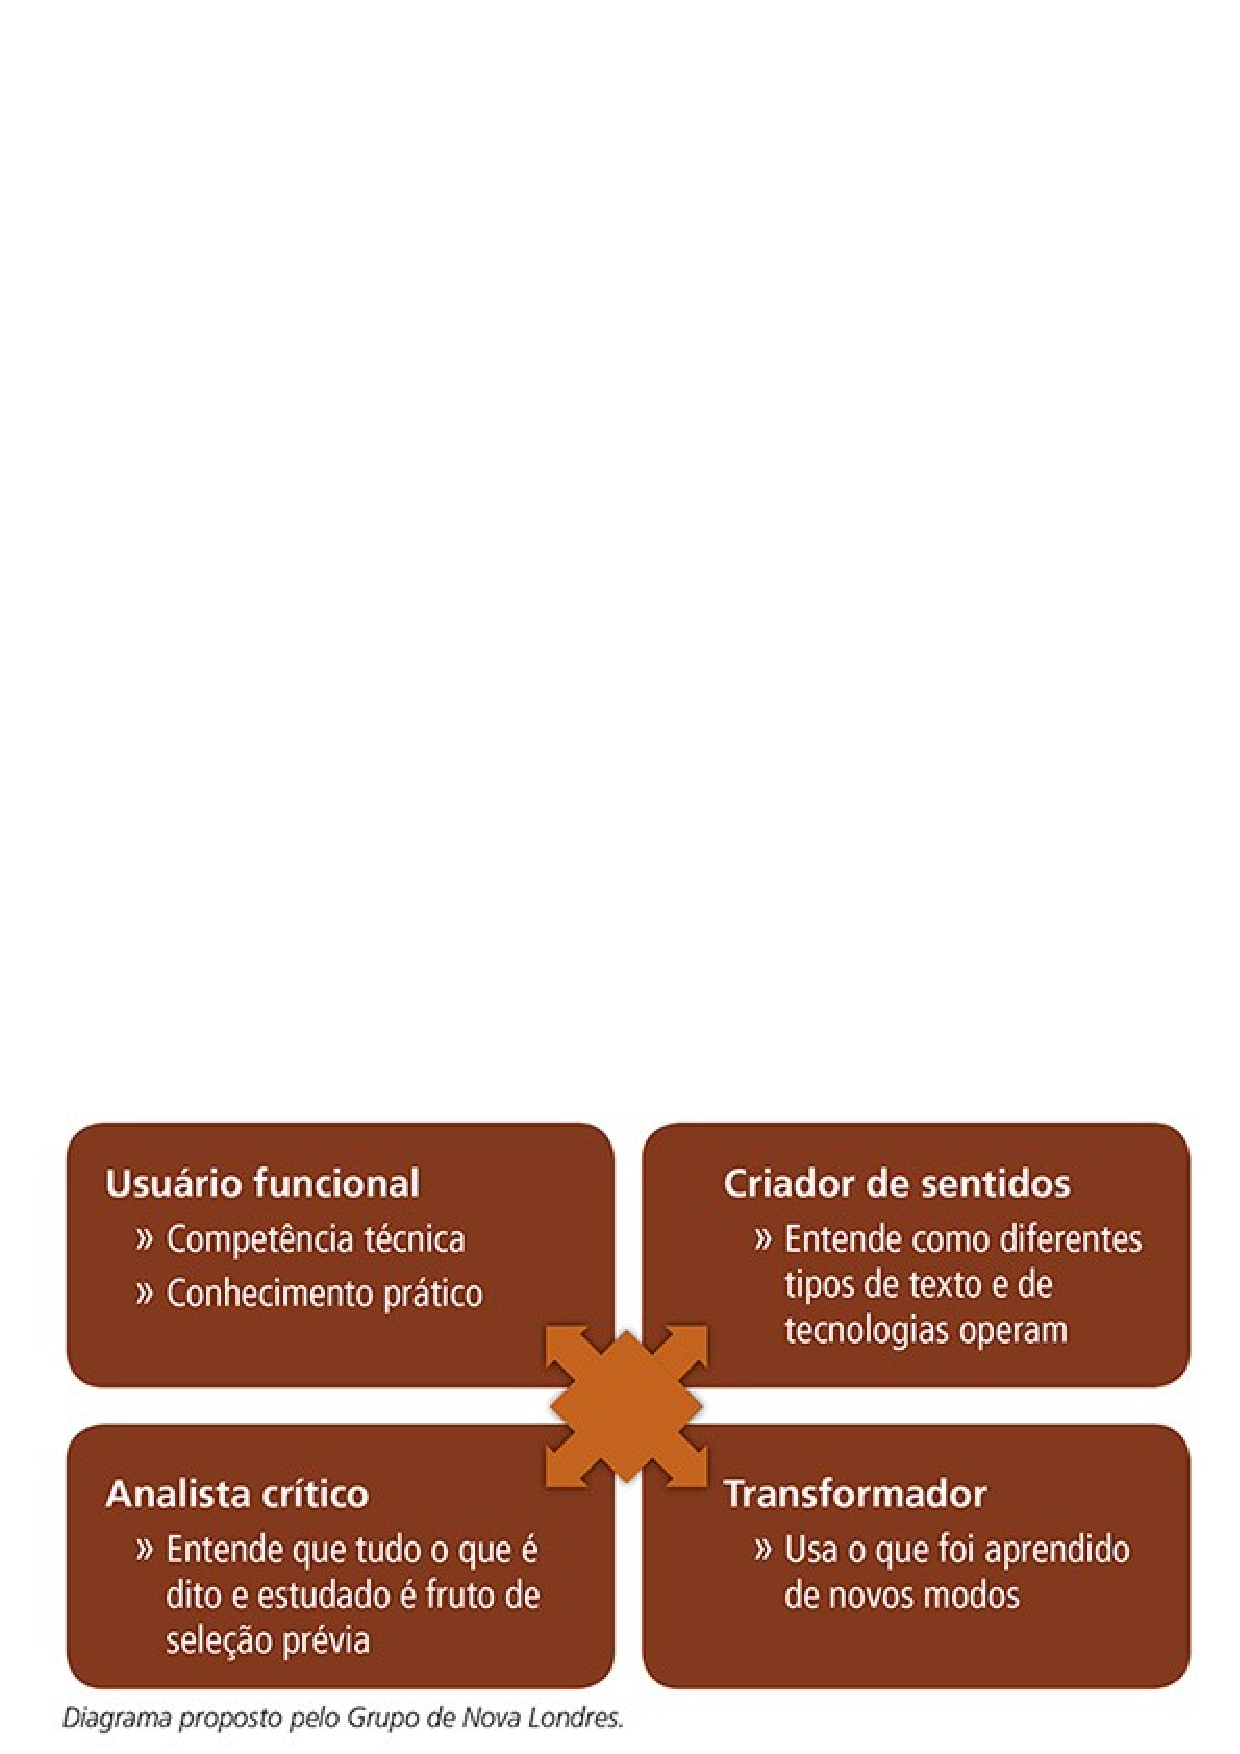
\includegraphics[width=0.5\textwidth]{figure01.png}
 \caption{Frecuencia de aparición del léxico especializado en el corpus.}
 \label{fig01}
 \source{elaboración própria.}
\end{figure}


\subsection{Léxico académico y resultados globales de la evaluación escrita}\label{sec-lex-aca-res}
En este apartado, la \Cref{fig02} da cuenta de la relación existente entre la
evaluaciónde los textos, considerando tanto el contenido como los aspectos
vinculados con laredacción, y la presencia de léxico académico. De los datos
obtenidos, se destaca que laslíneas para cada elemento son, en general,
bastante similares, pero con un promedio másbajo en el componente léxico. En
este sentido, destacan los resultados del estudiante 15,quien obtuvo el puntaje
total para ambas dimensiones, así como los puntajes delestudiante 32, que
obtuvo sobre el 80\% de logro tanto para la producción textual comopara el
léxico académico. A pesar de lo anterior, no podemos establecer una
relacióndirecta entre léxico académico y calidad textual, pues una
generalización de ese tipodejaría de lado las diferencias de puntaje que
evidencian los estudiantes 3, 7, 11, 19, 25 y35, quienes presentan una
distancia considerable entre el puntaje global de sus escritos yla presencia de
léxico académico.

\begin{figure}[htbp]
 \centering
 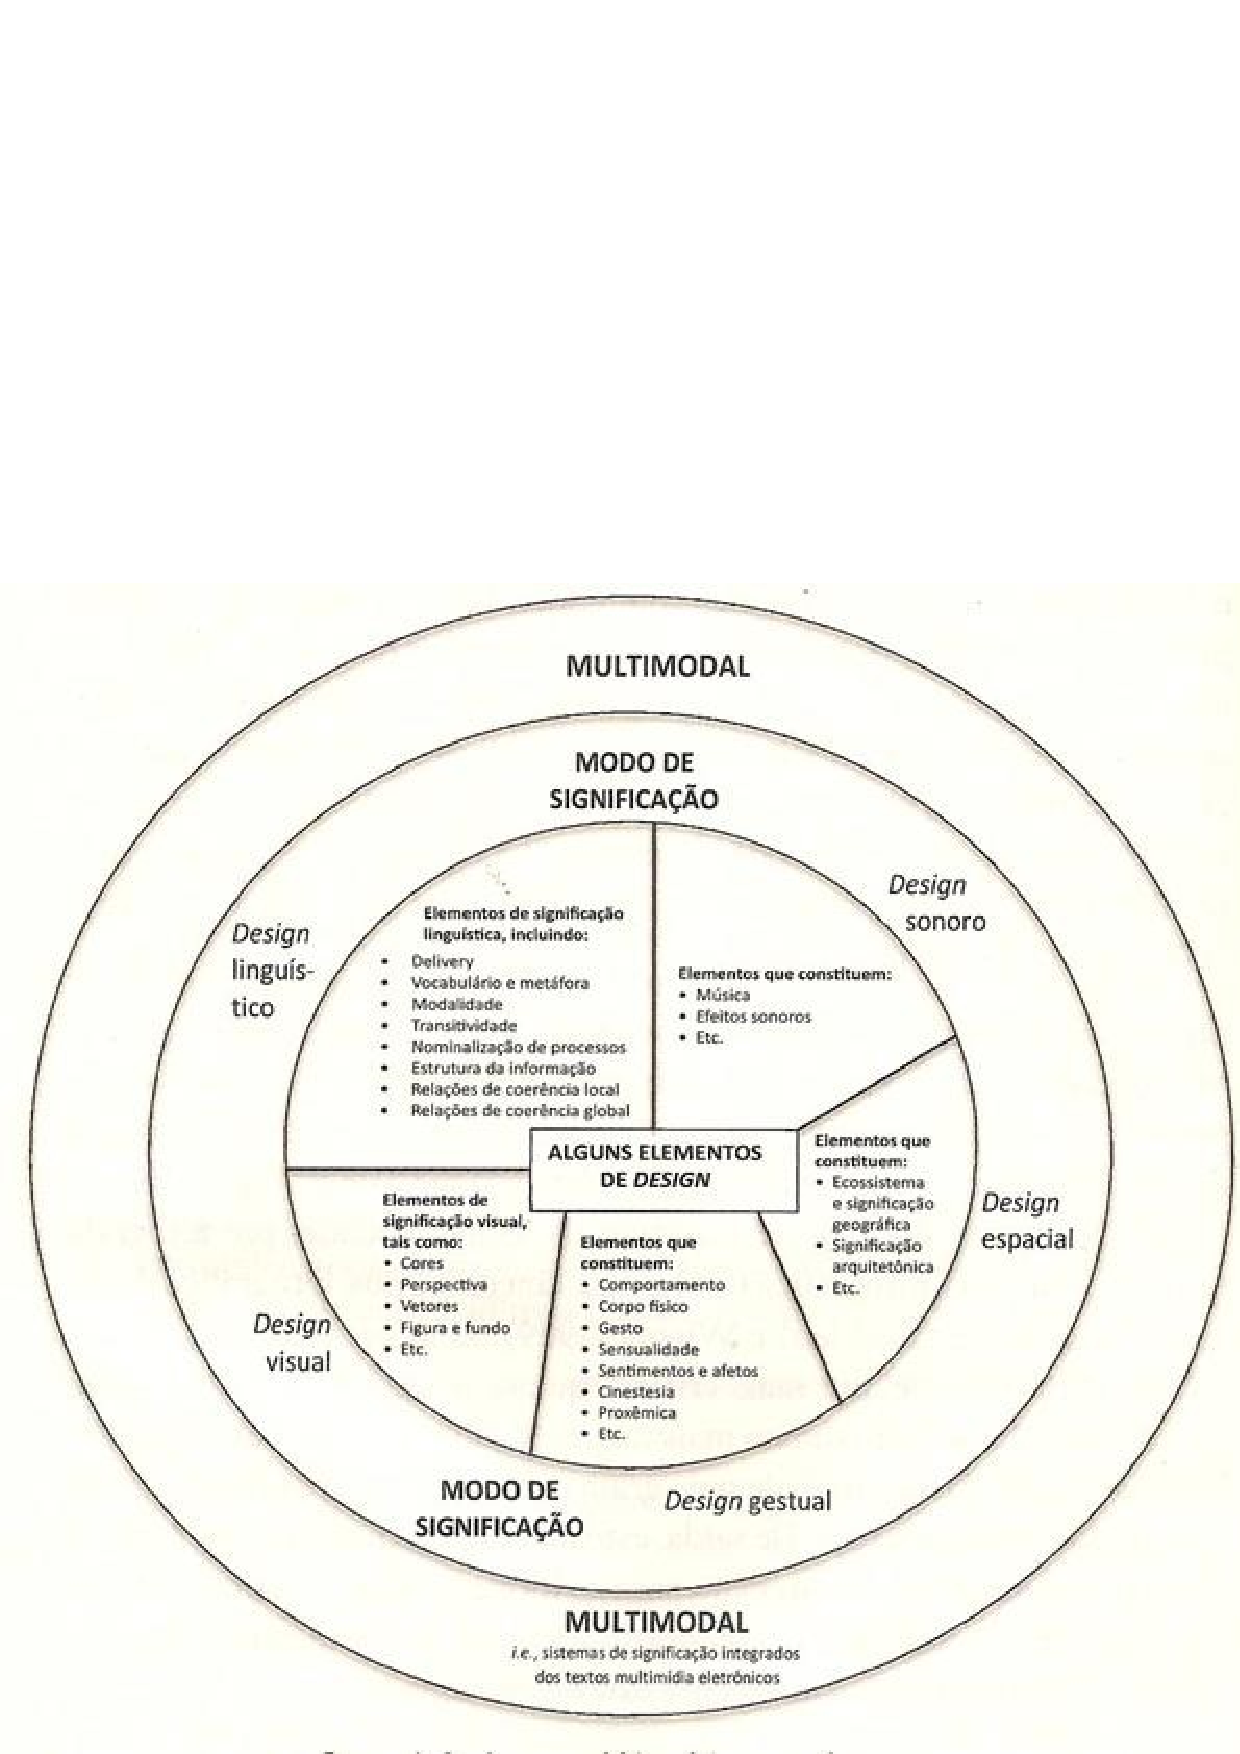
\includegraphics[width=0.6\textwidth]{figure02.png}
 \caption{Relación entre léxico académico y calidad global de los textos.}
 \label{fig02}
 \source{elaboración própria.}
\end{figure}


\subsection{Léxico académico y contenido de los textos}\label{sec-contenido}
En el caso del vínculo entre léxico académico y contenido de los textos,
seevidencia una relación bastante más estrecha (\Cref{fig03}). Se observa no solo
que laslíneas son más cercanas, sino también que los casos en los que existe
puntaje distanteson mucho menores: estudiantes 11, 17, 18, 19, 25 y 35.

Un caso particularmente llamativo es el del estudiante 25, quien obtuvo un
100\%de logro en el contenido, pero tan solo un 40\% en el componente léxico.
Esta diferenciapodría explicarse debido a que el método que utilizamos para
evaluar esta últimadimensión solo toma en cuenta la presencia de palabras
exactas, por tanto, la sinonimia,correferencia y otros mecanismos de cohesión
no fueron considerados. Esta idea serefuerza cuando volvemos a la \Cref{fig02},
pues se evidencia que el estudiante en cuestiónpresenta un alto nivel en la
calidad global de su escrito, lo que podría redundar en unvariado uso de
mecanismos de cohesión.

\begin{figure}[htbp]
 \centering
 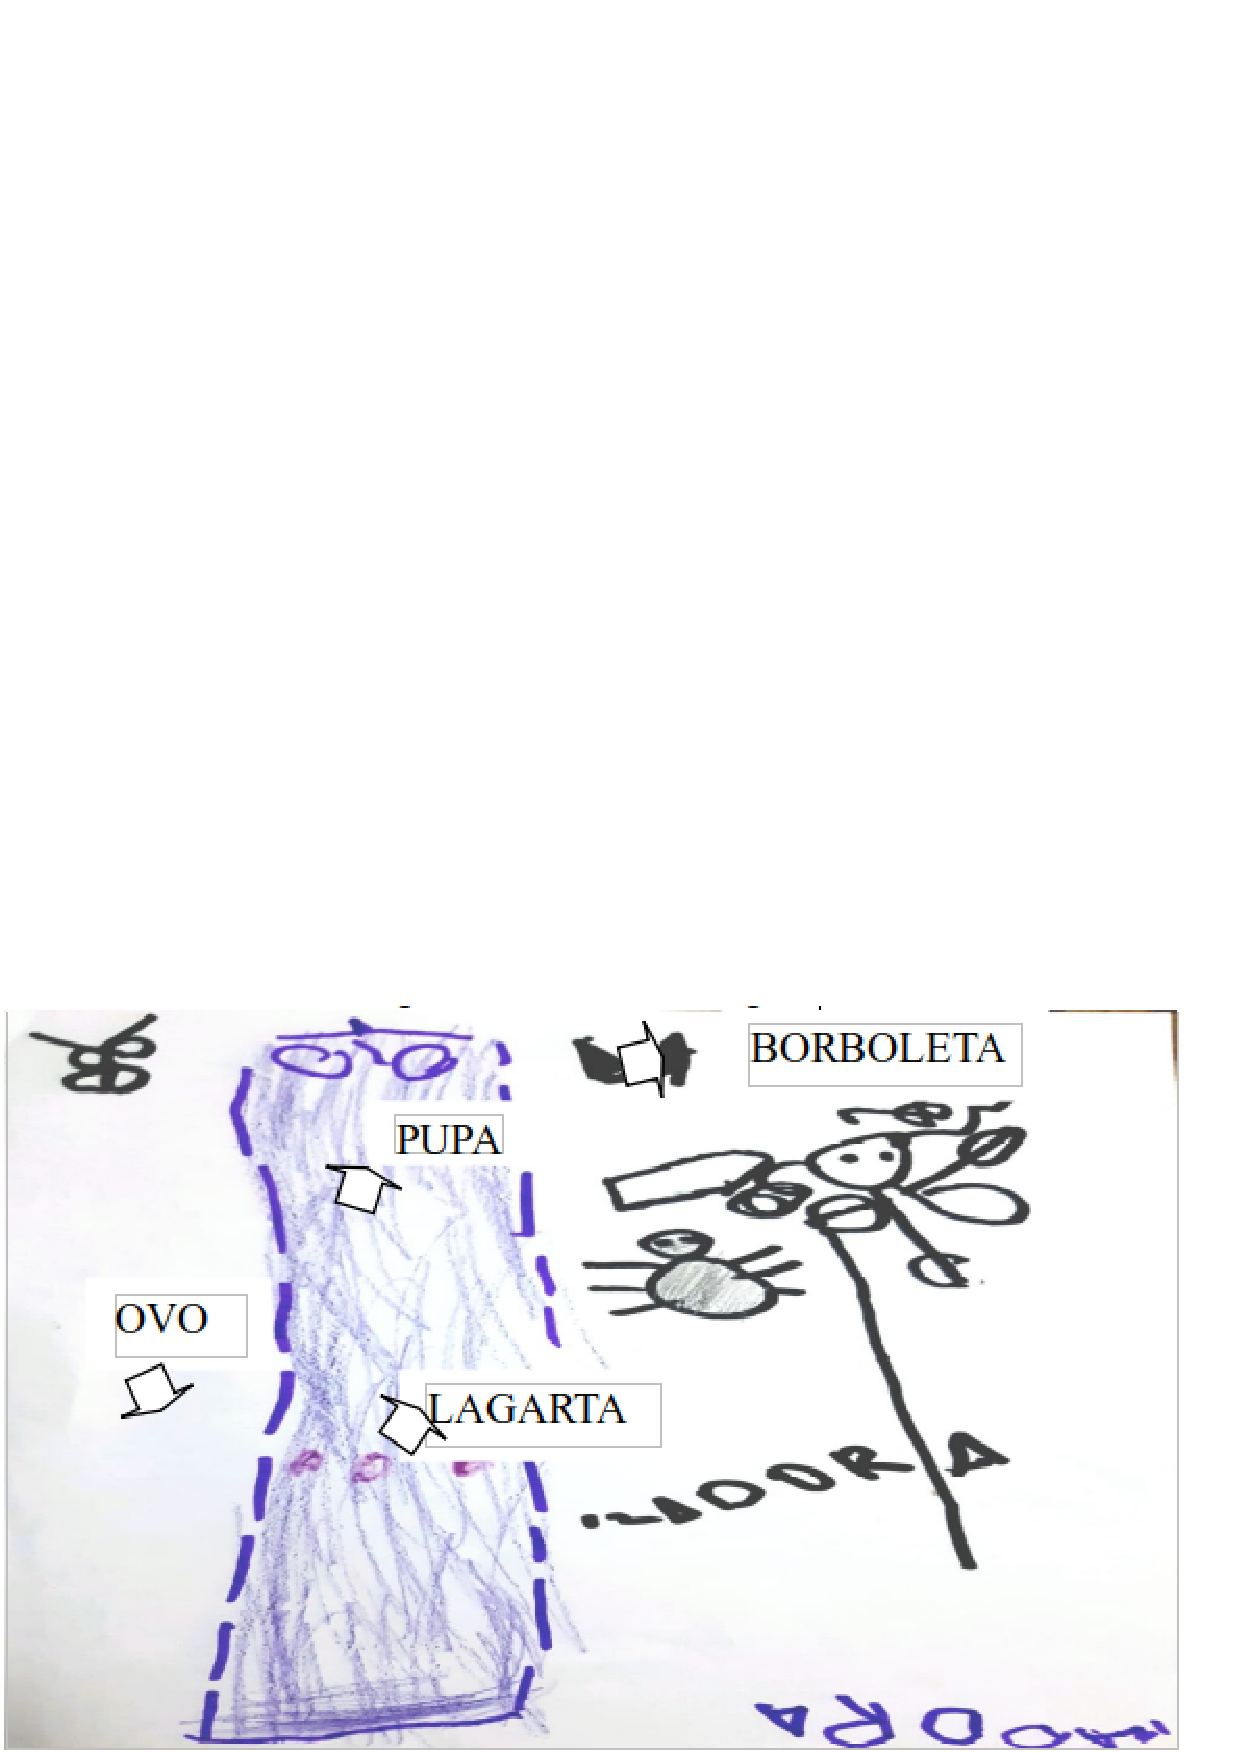
\includegraphics[width=0.6\textwidth]{figure03.png}
 \caption{Relación entre léxico académico y contenido de los textos.}
 \label{fig03}
 \source{elaboración própria.}
\end{figure}


\subsection{Léxico académico y calidad textual}\label{sec-calidad}
Respecto de esta relación, nos parece interesante destacar que no se
evidenciauna tendencia clara (\Cref{fig04}): por una parte, hay estudiantes que
demuestran resultadosmuy cercanos entre léxico académico y la calidad textual
de su escrito (1, 2, 5, 8, 15, 32);mientras que, por otra, algunos dan cuenta
de resultados bastante alejados (4, 5, 6, 11,17, 18, 19, 25, 30, 35).

\begin{figure}[htbp]
 \centering
 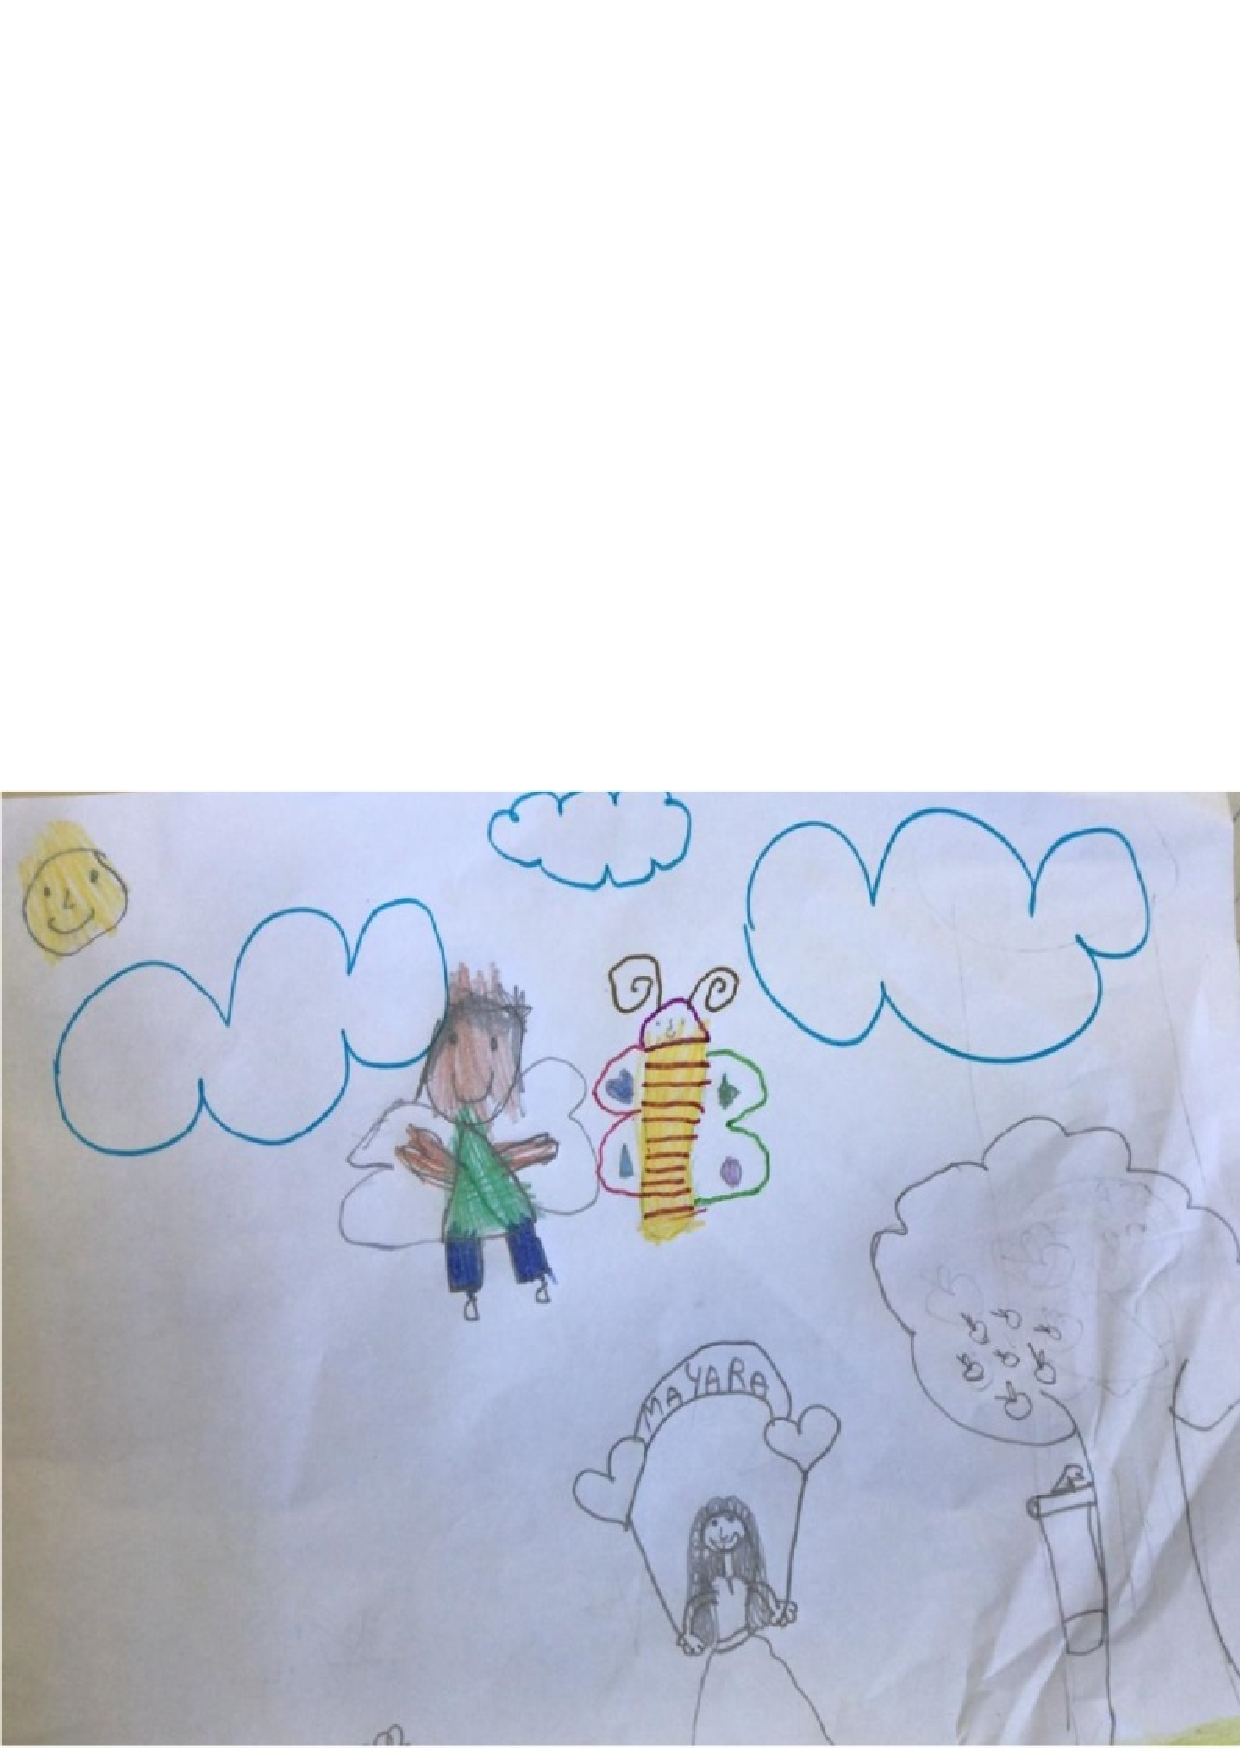
\includegraphics[width=0.6\textwidth]{figure04.png}
 \caption{Relación entre léxico académico y calidad textual.}
 \label{fig04}
 \source{elaboración própria.}
\end{figure}


\section{Discusión}\label{sec-discusion}
La relación entre competencia léxica y escritura ha sido profusamente estudiada
enel ámbito de la lengua inglesa y de la enseñanza de una segunda lengua. Si
nosenfocamos en el plano de la escritura académica, trabajos como el de \textcite{PrezCaado2010,Yoon2018,Pan2019}, 
entre muchos otros, se han centrado en
distintos aspectos de laescritura académica y su relación con la competencia
léxica: aprendizaje virtual ydesarrollo del léxico, desarrollo de la escritura
en L2 y presencia de lexical bundles entextos académicos, respectivamente. En
nuestra lengua, estudios sobre competencialéxica en la educación superior –
como el de \textcite{RiffoOcares2014,munoz2015,GonzaloZapico2016,Zapico2017,vega2018,Trigo2019},
entre otros muchos –, dan cuenta de la influencia que los estudiossobre
disponibilidad léxica han tenido en el ámbito de la educación a través de
lautilización de metodologías cuantitativas que miden el léxico mediante
evaluacionesespecíficas.

En contraste, más escasos resultan los trabajos que ponen el foco en el
léxicodesde una perspectiva integrada \cite[p. e.]{madrigal2016,gracia2019},
perspectiva que adopta también la presente investigación. Un aporte
interesante alrespecto es el que realizan \textcite{aravena}, quienes se
enfrentan al estudio delléxico en su contexto comunicativo y, sobre esa base,
relevan la importancia que tieneesta competencia en el desarrollo de
habilidades comunicativas complejas, como la adquisición de una segunda lengua
o el desempeño en lectura y escritura, desempeñoque incide directamente en el
rendimiento académico (p. 199). 

En cuanto a la relación entre dominio léxico y calidad textual, nos
pareceinteresante destacar que un texto con mayor riqueza léxica o, en el caso
del corpusanalizado, con mayor presencia de léxico académico, “no
necesariamente [...] va a estarbien realizado, pues habría que tomar en cuenta,
además, la cohesión y coherencia, eluso del componente notacional, así como la
puesta en práctica de requisitos gramaticalesnormativos” \cite[p. 145]{madrigal2016}.
Lo anterior se refuerza al observar loshallazgos de
\textcite{LilloFuentes2020}, quienes realizan una investigación en la
quevaloran la calidad de la escritura de trabajos finales de grado de una
carrera del área de laingeniería y la relacionan con rasgos
lingüístico-discursivos. En lo concerniente al vínculocalidad-riqueza léxica,
los autores señalan que “existeuna correlación negativa entre elnúmero de
palabras del escrito y la calidad de la escritura, por lo que las
introduccionesque poseen mayor extensión, tienden a catalogarse de baja
calidad” \cite[p. 11]{LilloFuentes2020}.

Tomando en cuenta lo anterior, tanto nuestra investigación como la de
estosautores parecen evidenciar que unidades léxicas con contenido no nocional,
comoconectores, pronombres, etc., tienen una mayor incidencia en aspectos como
la cohesión,lo que, a su vez, repercute directamente en la calidad de un texto.
En la misma línea, unainvestigación desarrollada hace varias décadas en un
contexto enseñanza de inglés comoL2 señala entre sus hallazgos que los ensayos
redactados por estudiantes cuyashabilidades de escritura se ubican en niveles
avanzados suelen tener un alto número deconectores y pronombres \cite{Reid1992}.
Esto podría explicar perfectamente los resultadosde estudiantes que, pese a
evidenciar un alto nivel de desempeño en su escritura, dancuenta de una baja
presencia en cuanto a léxico académico (e.g., estudiantes 4, 5, 6, 11,17, 18,
19, 25, 30, 35 en la \Cref{fig04}). Sin duda, esta reflexión invita a indagar en
larelación entre calidad textual y léxico no nocional en textos producidos por
estudiantesuniversitarios de nuevo ingreso.

Sobre esta base, más que confrontar los resultados del presente trabajo con
losque obtuvieron \textcite{RiffoOcares2014,Giammatteo2003,GonzaloZapico2016,Wood2019}
– entre otros en los que se
correlacionapositivamente la competencia léxica con diferentes aspectos de la
competenciacomunicativa (productiva y receptiva) –, nos inclinamos por destacar
que existe mayorincidencia del léxico académico en uno de los aspectos de la
competencia comunicativaescrita: el contenido textual.

Si bien estos resultados no son generalizables dadas las características
delestudio, es posible encontrar en la literatura una profusa cantidad de
trabajos querelacionan el léxico especializado con el dominio disciplinar,
sobre todo si consideramosen este ámbito lo mucho que se ha escrito sobre
alfabetización académica \cite{cantis2013,Baker2019,Kse2019}.
La relación que es posibleestablecer entre léxico académico, contenido
textual e incorporación de los aprendientesen una comunidad discursiva bien la
identifica \textcite[p. 55]{acevedo2006}, quien realiza unestudio en el que analiza
patrones léxicos en 163 trabajos de jóvenes universitarios yconcluye que la
utilización de terminología de cada especialidad da cuenta del “nivel
deespecialización alcanzado por los autores de los informes”.

En síntesis, los resultados de esta acotada experiencia nos entregan
informaciónvaliosa, desde el punto de vista pedagógico, sobre la importancia
que el léxico académico evidenció en el nivel de logro en el plano del
contenido de los textos, lo que, a su vez,incidió positivamente en la
evaluación global de los trabajos. Sin embargo, esta relaciónno llega a ser
determinante, pues hay antecedentes en la literatura especializada querelevan
una alta presencia de léxico no nocional en textos de alto nivel, lo que
podríaexplicar la distancia entre la calidad textual y el léxico disciplinar en
el corpus con el quehemos trabajado.



\section{Conclusiones}\label{sec-conclusiones}
Las analíticas de aprendizaje que hemos generado a través del software
Iramuteq – tanto la \Cref{fig01}, que da cuenta de la frecuencia del léxico
académico, como lasrestantes, que evidencian el desempeño en una tarea de
escritura –, nos permitenestablecer que los textos analizados presentan una
relación estrecha entre léxicoacadémico y calidad del contenido de los textos,
No obstante, a nivel de calidad textual(vale decir, considerando ortografía,
extensión, coherencia y cohesión y organización yestructura), la influencia del
léxico académico resulta menos determinante. Esto nos invitaa reflexionar en
torno al nivel de incidencia que el léxico no nocional (vale decir,conectores,
pronombres, preposiciones, etc.) tiene en la calidad de los textos, por lo
quese abre una interesante línea para futuros trabajos.

Finalmente, cabe precisar que, si bien el diseño de la investigación no nos
permitegeneralizar los resultados, estos ofrecen datos interesantes en lo
relativo a la importanciaque el desarrollo de la competencia léxica académica
posee en los procesos dealfabetización académica de los estudiantes
universitarios, sobre todo, considerando losindicios que entrega esta
competencia en relación con el dominio disciplinar.


\printbibliography\label{sec-bib}
% if the text is not in Portuguese, it might be necessary to use the code below instead to print the correct ABNT abbreviations [s.n.], [s.l.] 
%\begin{portuguese}
%\printbibliography[title={Bibliography}]
%\end{portuguese}

\end{document}
